% Options for packages loaded elsewhere
\PassOptionsToPackage{unicode}{hyperref}
\PassOptionsToPackage{hyphens}{url}
\PassOptionsToPackage{dvipsnames,svgnames,x11names}{xcolor}
%
\documentclass[
  authoryear]{elsarticle}

\usepackage{amsmath,amssymb}
\usepackage{iftex}
\ifPDFTeX
  \usepackage[T1]{fontenc}
  \usepackage[utf8]{inputenc}
  \usepackage{textcomp} % provide euro and other symbols
\else % if luatex or xetex
  \usepackage{unicode-math}
  \defaultfontfeatures{Scale=MatchLowercase}
  \defaultfontfeatures[\rmfamily]{Ligatures=TeX,Scale=1}
\fi
\usepackage{lmodern}
\ifPDFTeX\else  
    % xetex/luatex font selection
\fi
% Use upquote if available, for straight quotes in verbatim environments
\IfFileExists{upquote.sty}{\usepackage{upquote}}{}
\IfFileExists{microtype.sty}{% use microtype if available
  \usepackage[]{microtype}
  \UseMicrotypeSet[protrusion]{basicmath} % disable protrusion for tt fonts
}{}
\makeatletter
\@ifundefined{KOMAClassName}{% if non-KOMA class
  \IfFileExists{parskip.sty}{%
    \usepackage{parskip}
  }{% else
    \setlength{\parindent}{0pt}
    \setlength{\parskip}{6pt plus 2pt minus 1pt}}
}{% if KOMA class
  \KOMAoptions{parskip=half}}
\makeatother
\usepackage{xcolor}
\setlength{\emergencystretch}{3em} % prevent overfull lines
\setcounter{secnumdepth}{5}
% Make \paragraph and \subparagraph free-standing
\ifx\paragraph\undefined\else
  \let\oldparagraph\paragraph
  \renewcommand{\paragraph}[1]{\oldparagraph{#1}\mbox{}}
\fi
\ifx\subparagraph\undefined\else
  \let\oldsubparagraph\subparagraph
  \renewcommand{\subparagraph}[1]{\oldsubparagraph{#1}\mbox{}}
\fi


\providecommand{\tightlist}{%
  \setlength{\itemsep}{0pt}\setlength{\parskip}{0pt}}\usepackage{longtable,booktabs,array}
\usepackage{calc} % for calculating minipage widths
% Correct order of tables after \paragraph or \subparagraph
\usepackage{etoolbox}
\makeatletter
\patchcmd\longtable{\par}{\if@noskipsec\mbox{}\fi\par}{}{}
\makeatother
% Allow footnotes in longtable head/foot
\IfFileExists{footnotehyper.sty}{\usepackage{footnotehyper}}{\usepackage{footnote}}
\makesavenoteenv{longtable}
\usepackage{graphicx}
\makeatletter
\def\maxwidth{\ifdim\Gin@nat@width>\linewidth\linewidth\else\Gin@nat@width\fi}
\def\maxheight{\ifdim\Gin@nat@height>\textheight\textheight\else\Gin@nat@height\fi}
\makeatother
% Scale images if necessary, so that they will not overflow the page
% margins by default, and it is still possible to overwrite the defaults
% using explicit options in \includegraphics[width, height, ...]{}
\setkeys{Gin}{width=\maxwidth,height=\maxheight,keepaspectratio}
% Set default figure placement to htbp
\makeatletter
\def\fps@figure{htbp}
\makeatother

\makeatletter
\@ifpackageloaded{caption}{}{\usepackage{caption}}
\AtBeginDocument{%
\ifdefined\contentsname
  \renewcommand*\contentsname{Table of contents}
\else
  \newcommand\contentsname{Table of contents}
\fi
\ifdefined\listfigurename
  \renewcommand*\listfigurename{List of Figures}
\else
  \newcommand\listfigurename{List of Figures}
\fi
\ifdefined\listtablename
  \renewcommand*\listtablename{List of Tables}
\else
  \newcommand\listtablename{List of Tables}
\fi
\ifdefined\figurename
  \renewcommand*\figurename{Figure}
\else
  \newcommand\figurename{Figure}
\fi
\ifdefined\tablename
  \renewcommand*\tablename{Table}
\else
  \newcommand\tablename{Table}
\fi
}
\@ifpackageloaded{float}{}{\usepackage{float}}
\floatstyle{ruled}
\@ifundefined{c@chapter}{\newfloat{codelisting}{h}{lop}}{\newfloat{codelisting}{h}{lop}[chapter]}
\floatname{codelisting}{Listing}
\newcommand*\listoflistings{\listof{codelisting}{List of Listings}}
\makeatother
\makeatletter
\makeatother
\makeatletter
\@ifpackageloaded{caption}{}{\usepackage{caption}}
\@ifpackageloaded{subcaption}{}{\usepackage{subcaption}}
\makeatother
\journal{JIMR}
\ifLuaTeX
  \usepackage{selnolig}  % disable illegal ligatures
\fi
\usepackage[]{natbib}
\bibliographystyle{elsarticle-harv}
\usepackage{bookmark}

\IfFileExists{xurl.sty}{\usepackage{xurl}}{} % add URL line breaks if available
\urlstyle{same} % disable monospaced font for URLs
\hypersetup{
  pdftitle={Beyond the paradox of interoperability in open health data standards},
  pdfauthor={Daniel Kapitan; Melle Sieswerda; Andre Dekker},
  pdfkeywords={OMOP, OpenEHR, FHIR, secondary use, data
platform, digital platform},
  colorlinks=true,
  linkcolor={blue},
  filecolor={Maroon},
  citecolor={Blue},
  urlcolor={Blue},
  pdfcreator={LaTeX via pandoc}}

\setlength{\parindent}{6pt}
\begin{document}

\begin{frontmatter}
\title{Beyond the paradox of interoperability in open health data
standards}
\author[1,2,3]{Daniel Kapitan%
%
}
 \ead{daniel@kapitan.net} 
\author[4,5]{Melle Sieswerda%
%
}

\author[5]{Andre Dekker%
%
}


\affiliation[1]{organization={Dutch Hospital
Data},city={Utrecht},country={the
Netherlands},countrysep={,},postcodesep={}}
\affiliation[2]{organization={PharmAccess
Foundation},city={Amsterdam},country={the
Netherlands},countrysep={,},postcodesep={}}
\affiliation[3]{organization={Eindhoven University of
Technology},city={Eindhoven},country={the
Netherlands},countrysep={,},postcodesep={}}
\affiliation[4]{organization={Integral Cancer Registry
Netherlands},city={Eindhoven},country={the
Netherlands},countrysep={,},postcodesep={}}
\affiliation[5]{organization={Maastricht
University},city={Maastricht},country={the
Netherlands},countrysep={,},postcodesep={}}

\cortext[cor1]{Corresponding author}



        
\begin{abstract}
In response to the proposal of Tsafnat et al.~to converge towards three
open health data standards, we discuss two specific contexts, namely
standardization of i) health data for federated learning, and ii) health
data sharing in low- and middle income countries (LMICs). Based on our
ongoing work in both areas, we provide a critical reflection on the
proposed alignment of using OpenEHR, FHIR and OMOP as the default
standard for the three domains of clinical care and administration, data
exchange and longitudinal analysis, respectively. We find that for the
two contexts considered there, this trichotomy does not do justice to
details that are crucial in real-world implementations. This perspetive
describes more specific design principles and implementation choices for
these two types of health data sharing. In both case, we observe a
strong convergence towards FHIR, while OMOP is used as an alternative or
in combination with FHIR for federated learning.
\end{abstract}





\begin{keyword}
    OMOP \sep OpenEHR \sep FHIR \sep secondary use \sep data
platform \sep 
    digital platform
\end{keyword}
\end{frontmatter}
    
\section{Looking beyond the paradox of
interoperability}\label{looking-beyond-the-paradox-of-interoperability}

``A paradox of health care interoperability is the existence of a large
number of standards exists with significant overlap among them,'' say
Tsafnat et al., followed by a call to actions towards the health
informatics community to put effort into establishing convergence and
preventing collision \citep{tsafnat2024converge}. To do so, they propose
to converge on three open standards, namely i) OpenEHR for clinical care
and administration; ii) Fast Health Interoperability Resources (FHIR)
for data exhange and iii) Observational Medical Outcomes Partnership
Common Data Model (OMOP) for longitudinal analysis. They argue that open
data standards, backed by engaged communities, hold an advantage over
proprietary ones and therefore should be chosen as the steppingstones
towards achieving true interoperability.

While we support their high-level rationale and intention, we feel their
proposed trichotomy does not do justice to details that are crucial in
real-world implementations. This viewpoint provides a critical
reflection on the their proposed framework in three parts. First, we
reflect on salient differences between the three open standards from the
perspective of the notion of openness of digital platforms
\citep{dereuver2018digital}, data platforms \citep{dereuver2022openness}
and the paradox of open \citep{keller2021paradox}. Subsequently, we
present our findings in designing and implementing health data platforms
in two specific contexts, namely i) platforms for federated learning on
shared health data; and ii) health data platforms for low and middle
income countries (LMICs). We conclude with \ldots{}

\section{The paradox of open for health data
standards}\label{the-paradox-of-open-for-health-data-standards}

Besides the paradox of interoperability put forward by Tsafnat et al.,
we argue that although open standards are a necessary, but not
sufficient condition for convergence of health data standarization. We
posit that open source implementations of components, libraries etc.
constitute another necessary condition for establishing a flourishing
health data platform and associated ecosystem. Research on digital
platforms underline the importance of the platform openness, not only in
term of open standards, but also in term of extensibility of the code
base, availibility of complements to the core technical platform (in our
case the data standard itself) and availibility of executable pieces of
software \citep{dereuver2018digital}. Only when these aspects of digital
platforms are fullfilled can we resonably expect that the platform will
indeed be longlived.

In what they call the paradox of open, Keller and Tarkowsi argue that
this conventional approach of open standards and open source flourish
under two types of conditions \citep{keller2021paradox}. First, projects
where many people contribute to the creation of a common resource have
proven succesful. This is the story of Wikipedia, OpenStreetMap,
Blender.org, and the countless free software projects that provide much
of the internet's infrastructure. Indeed, Tsafnat et al.~have explicitly
taken into account that ``an engaged and vibrant community is a major
advantage for the longevity of the data standards it uses,'' which has
informed their proposal to converge towards OMOP, FHIR en OpenEHR.
However, the emphasis on open source implementations is somewhat
overlooked. This point is only mentioned in passing and indirectly, when
Tsafnat et al.~reference work done by Reynolds and Wyatt who already
argued in 2011 ``\ldots{} for the superiority of open source licensing
to promote safer, more effective health care information systems. We
claim that open source licensing in health care information systems is
essential to rational procurement strategy'' \citep{reynolds2011open}.
We believe that a realistic assessment of the current position of an
open standard within the wider context of availability of complementary
components and open source implementations is equally important when
choosing which standard to adopt.

This point is related to the second condition put forward by Keller and
Tarkoswki, namely that the conventional open approach has proven
fruitful when ``opening up'' is the result of external incentives or
requirements, rather than voluntary actions. This is the story of
publicly-funded knowledge production like Open Access academic
publications, cultural heritage collections in the Public Domain, Open
Educational Resources (OER), and Open Government data. A canonical
example in the birth of the GSM standard, which was mandated by European
legislation.\footnote{See
  \url{https://en.wikipedia.org/wiki/GSM\#Initial_European_development}
  for details.} Reflecting on this perspective on openness, we observer
a salient difference between FHIR vis-a-vis OpenEHR and OMOP, namely
that the former is the only one that has been mandated (or at least
strongly recommended) in some jurisdictions. In the US, the Office of
the National Coordinator for Health Information Technology (ONC) and the
Centers for Medicare and Medicaid Services (CMS) has introduced a steady
stream of new regulations, criteria, and deadlines in Health IT that has
resulted in significant adoption of FHIR \citep{firely2023fhir}. In
India, the open Health Claims Exchange protocol specification - which is
based on FHIR - has been mandated by the Indian government as the
standard for e-claims handling \citep{hcx}. The African Union recommends
all new implementations and digital health system improvements use FHIR
as the primary mechanism for data exchange \citep{tilahun2023african},
but doesn't say anything about the use of, for example, OpenEHR for
administrative systems of record.

These external incentives have resulted in a large boost in both
commercial and open source development activities in the FHIR ecosystem.
One such example is the speed with which the Bulk FHIR API has been
defined and implemented in almost all major implementations
\citep{mandl2020push, jones2021landscape}. It has also led to more
people voluntarily contributing to FHIR-related open source projects,
which has resulted in a wide offering of FHIR components across major
technology stacks (Java, Python, .NET), thereby strengthening the first
condition. By comparison, the ecosystem of OMOP and OpenEHR is have not
yet profited from external incentives to grow their community \ldots{}

\begin{itemize}
\tightlist
\item
  smaller than that of FHIR
\item
  The majority of OMOP components are run by Observational Health Data
  Science and Informatics (OHDSI) \ldots Say something that OMOP still
  has a relatively large ecosystem, with R libraries, pyOMOP etc.
\item
  The OpenEHR, however, seems subscritical. We are not judging the
  content and approach of OpenEHR, but there are just so few
  implementations.
\end{itemize}

Hence, we stress that beyond the evaluating the intrinic structure of an
open standard (which one is most suitable for a given domain) and the
community that supports the standard, we need to take into account the
wider ecosystem of open source implementations, complementary components
etc. From this wider perspective on the whole ecosystem around a
standard, FHIR stands out as having the diverse and rich ecosystem
because it has been mandated in certain jurisdictions. This is relevant
when comparing these standards in real-world implementations.

\section{Standarization of health data for federated
learning}\label{standarization-of-health-data-for-federated-learning}

The current fragmentation in health data is one of the major barriers
towards leveraging the potential medical data for machine learning (ML).
Without access to sufficient data, ML will be prevented from reaching
its full potential and, ultimately, from making the transition from
research to clinical practice. Data like this is hard to obtain, because
health data is highly sensitive and its usage is tightly regulated.

Federated learning (FL) is a learning paradigm that aims to address
these issues of data governance and privacy by training algorithms
collaboratively without exchanging the data itself
\citep{rieke2020future, teo2024federated}. Based on ongoing work with
the PLUGIN healthcare consortium (\url{https://plugin.healthcare}, in
Dutch) we have detailed an architecture for FL for secondary use. To
this purpose, the the National Health Data Infrastructure agreements for
research, policy and innovation for the Dutch healthcare sector which
have been adopted at the beginning of 2024, has been taken as the
starting point \citep{healthri2024agreements}.
Figure~\ref{fig-healthri-architecture} shows a high level overview of
the platform, which comprises three areas (multiple use, applications
and generic features) and a total of 26 functional components (for
details please refer to \citep{healthri2024agreements}).

\begin{figure}

\centering{

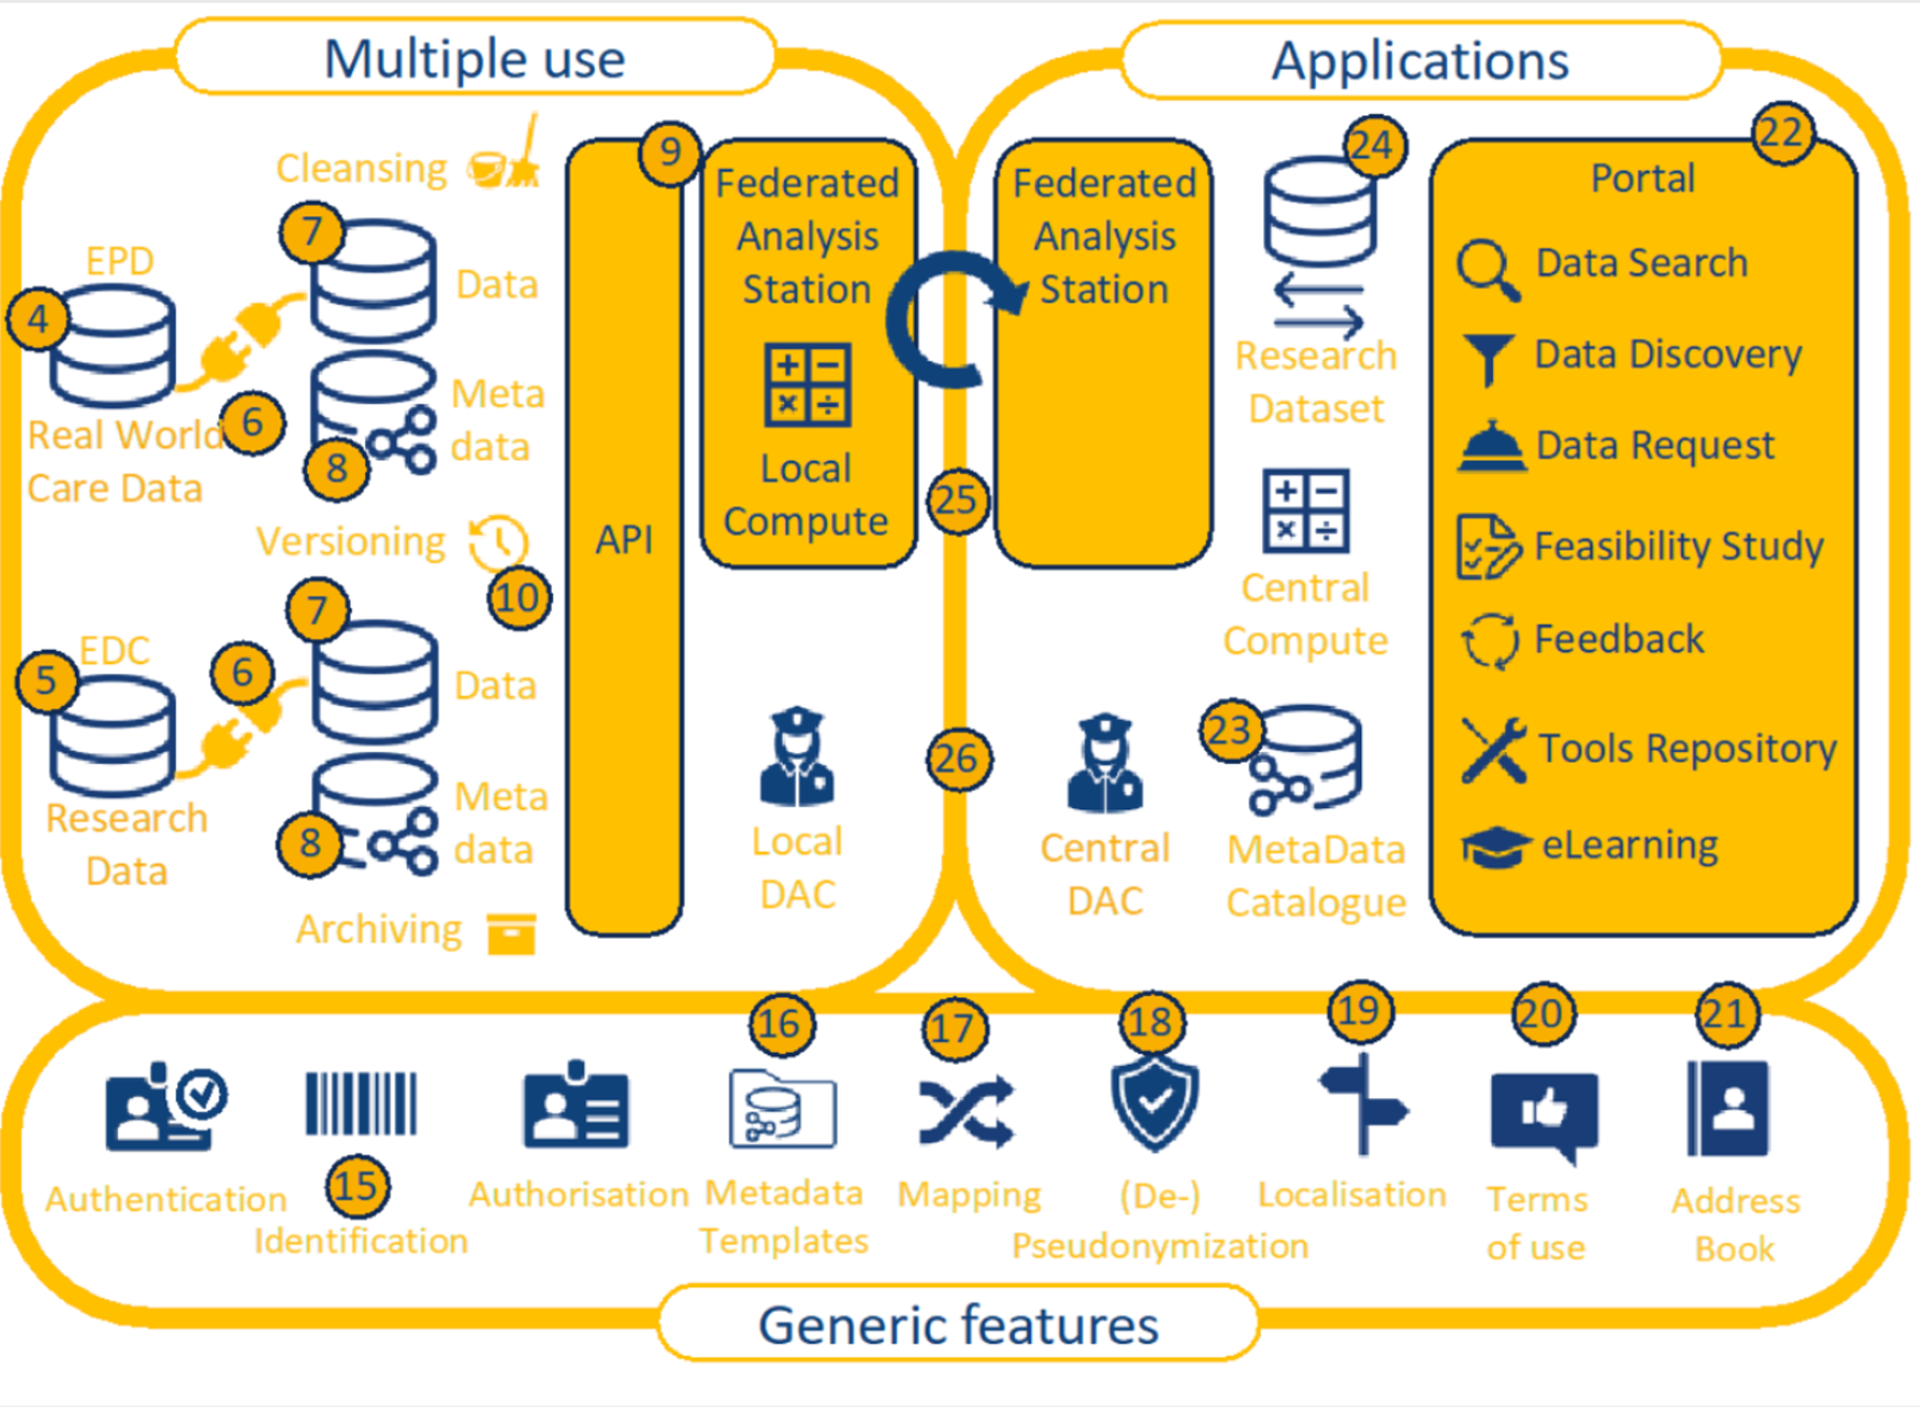
\includegraphics{health-ri-architecture.png}

}

\caption{\label{fig-healthri-architecture}Reference architecture for the
Dutch health data infrastructure for research and innovation
\citep{healthri2024agreements}}

\end{figure}%

The principle of FL has been actively researched and developed within
the Dutch healthcare community. The first proof-of-concept of the
so-called Personal Health Train \citep{vansoest2018using} ultimately led
to the open source vantage6 platform \citep{smits2022improved}. One of
the prerequisites of this architecture is that organizations that
participate in a federation of `data stations' use the same common data
model (CDM) to make the data Findable, Accessible, Interoperable and
Resusable. These FAIR data stations comprise components 7, 8 and 9 in
Figure~\ref{fig-healthri-architecture}, i.e.~the data, metadata and
APIs, respectively, through which this the data station can be accessed
and used. FHIR has been chosen as the common data model quite early in
the development because of its practicality, provenance of RESTful APIs
out of the box, support of many healthcare terminologies and flexibility
through the profiling mechanims \citep{choudhury2020personal}.

This solution design has gained traction since then. The CODA platform,
which aims to implement a FL infrastructure in Canada, compared OMOP and
FHIR and chose the latter as it has been found to support more granular
mappings required for analytics \citep{mullie2023coda}. Given that
conceptually OMOP can be viewed as a strict subset of FHIR, hybrid
solutions using OMOP and FHIR combined have also been reported, such as
the German KETOS platform \citep{gruendner2019ketos} and the preliminary
findings from the European GenoMed4All project which aims to connect
clinical and -omics data \citep{cremonesi2023need}.

Using FHIR as the CDM in a FL architecture for persistent storage for
longitudinal analysis may strike many as counterintuitive. The fact that
some recent studies the practical designs of such platforms only mention
OMOP only attests to this misconception \citep{wong2022applying}.

\begin{itemize}
\item
  we don't say you can't use OMOP for data stations, in fact the
  following projects do that:

  \begin{itemize}
  \tightlist
  \item
    OHDSI analytics \citep{khalid2021standardized}
  \item
    \ldots{} (look for more)
  \end{itemize}
\item
  this distinction become irrelevant as OMOP will have FHIR interfaces,
  see https://omoponfhir.org
\item
  however, FHIR is the CDM we choose because it is a superset, allowing
  for example also administrative and claims data or claims data can't
  fit in OMOP
\item
  Principle of FHIR Profiles can be tied to principle of late binding:
  allow ingest of widely different sources, and gradually but more
  constraints and validations as you move closer to a specific use case.
  If machine learning is the primary objective for secondary use, we
  want to be able to cast a wider net of relevant data, rather than
  having very detailed data
\item
  Add more arguments here \ldots{}
\end{itemize}

\section{Health data standards in low- and middle income
countries}\label{health-data-standards-in-low--and-middle-income-countries}

The OpenHIE framework \citep{openhie} has been adopted by many
sub-Saharan African countries \citep{mamuye2022health} as the
architectural blueprint for implementing nation-wide health information
exchanges (HIE), including Nigeria \citep{dalhatu2023paper}, Kenya
\citep{thaiya2021adoption} and Tanzania \citep{nsaghurwe2021one}.
Conceptually, the OpenHIE framework constitutes a framework for an open
digital platform, that mostly focuses on transactional exchange of data,
that is, primary data sharing. Given the need to also enable secondary
data sharing for academic research, real-world evidence studies etc.,
African countries have, as a matter of course, extended the framework to
include ``data \& analytics services'' as an additional domain.

Based on our direct involvement in implementing and designing health
data platforms in these countries, we observed that FHIR was practically
the only viable solution. Although FHIR is originally intened for
creating a longitudinal database, in fact open source FHIR
implementations such as the HAPI FHIR server are the most widely used
standards for realizing the so-called Shared Health Record within the
OpenHIE architecture. not intended for

In relation to the conventional perspective on `openness', which
originally focused on open source and open standards as discussed above,
has been superseded by ``\ldots{} conflicts about privacy, economic
value extraction, the emergence of artificial intelligence, and the
destabilizing effects of dominant platforms on (democratic) societies.
Instead of access to information, the control of personal data has
emerged in the age of platforms as the critical contention''
\citep{keller2021paradox}. These conflicts are particularly salient in
the healthcare domain, where people are generally willing to share their
health data to receive the best care (primary use), while the attitude
towards secondary use of health data varies greatly depending on the
type and context \citep{cascini2024health}. Case studies on digital
platforms in healthcare point to an emerging pattern where the focus
shifts from the digital platform with its defining software and hardware
components, to the data as the primary object of interest in and of
itself \citep{ozalp2022digital, alaimo2022organizations}. This
observation ties into with the proposed research agenda by de Reuver et
al.~to consider data platforms as a phenomenon distinct from digital
platforms \citep{dereuver2018digital, dereuver2022openness}.

Essentially, ``\ldots{} this paradox is that openness of data is both a
challenge to and an enabler of concentrations of power. The ideas of
open access and free reuse of information goods continue to be some of
the most powerful challenges to the exclusive control by corporations
and states over information goods. Yet making such resources open also
exposes them to the imbalances of power that shape these societies --
and in the worst cases serves to strengthen these imbalances.'' Put
differently, having open standards is no guarantee that we will be able
to breakthrough the current status quo with huge asymmetries in terms of
bargaining power, access control and development resources related to
health data sharing. We posit that having open data standards is a
necessary condition in improving the current state of affairs, yet it is
not a sufficient condition.

The shift in perspective from digital platforms supporting primary data
sharing toward data platforms supporting secondary data sharing is a
contentious issue both in high income countries, with for example the
ongoing efforts to establish a European Health Data Space
\citep{otto2022designing}, and low- and middle income countries that are
aiming to deploy nationwide health information exchanges to support
primary and secondary data use at once \citep{mamuye2022health}. A
better understanding of openness is particularly relevant if we are to
realize a solidarity-based approach to health data sharing that i) gives
people a greater control over their data as active decision makers; ii)
ensures that the value of data is harnessed for public good; and iii)
moves society towards equity and justice by counteracting dynamics of
data extraction
\citep{kickbusch2021lancet, prainsack2022data, prainsack2023beyond}.

More than a decade later, we observe that only a very small fraction of
health IT systems are based on open source, the majority of which are
used in LMICs which we will discuss later \citep{digitalpublicgoods}.

\section{Conclusion and outlook}\label{conclusion-and-outlook}

\begin{itemize}
\tightlist
\item
  We underline the need for open data standards as a necessary condition
  to achieve interoperability
\item
  It is not a sufficient condition
\item
  MPC as next step up from FL
\end{itemize}


  \bibliography{plugin.bib}


\end{document}
